\documentclass[12pt,a4paper]{report}

\usepackage[spanish]{babel}
\usepackage[utf8]{inputenc}
\usepackage{dad}
\usepackage{pdfpages}

\title{Desarrollo de Aplicaciones Distribuidas: \\ Registrador de juegos}
\author{Rafael Gálvez-Cañero, Andreas Gerstmayr}
\date{Iteración 5 - 28 de Abril de 2015} % delete this line to display the current date



%%% BEGIN DOCUMENT
\begin{document}
\maketitle
\tableofcontents
\listoffigures
\listoftables

\pagenumbering{arabic}

% Esto representa la primera iteración (capítulo), información general
\chapter{Datos generales}

\section{Miembros del grupo}

\begin{table}[htdp]
\begin{center}
\begin{tabular}{|l|l|l|c|}
\hline
\textbf{Apellidos}&\textbf{Nombre}&\textbf{Correo-e}&\textbf{Grupo}\\
\hline
Gálvez-Cañero&Rafael&\href{mailto:galvesband@gmail.com}{galvesband@gmail.com}&18\\
Gerstmayr&Andreas&\href{mailto:andreas.gerstmayr@gmail.com}{andreas.gerstmayr@gmail.com}&18\\
\hline
\end{tabular}
\end{center}
\caption{Miembros del grupo}
\label{tab:miembros}
\end{table}%


\section{Descripción del sistema}

\begin{itemize}
\item \textbf{Tipo de sistema distribuido}:
\item \textbf{Nombre del proyecto}: Plataforma de juegos, Game Register
\item \textbf{Breve descripción}: Sub-sistema para registrar sesiones de juego e información asociada.
\end{itemize}

\subsection{Funcionalidad observable}

\begin{itemize}
\item Registrar el inicio y el término de todas las sesiones de juego.
\item Visualizar el historial de juegos.
\item Visualizar qué jugadores juegan en este momento.
\end{itemize}

\subsection{Servicios ofrecidos}
\begin{itemize}
\item Servicio de Registro: Capacidad de aceptar la información de una sesión de juego.
\item Servicio de Historial: Ofrece métodos para consultar el historial de sesiones.
\item Servicio de Sesiones Online: Muestra una lista de jugadores actualmente en activo.
\end{itemize}

\subsection{Servicios demandados}
\begin{itemize}
\item Servicio X: breve descripción. Fecha aproximada a partir de la que se necesitará (si se conoce).
\item Servicio Y: idem.
\end{itemize}

\section{Direcciones de descarga y planificación}

\begin{table}[htdp]
\begin{center}
\begin{tabular}{|c|c|}
\hline
\textbf{Código fuente}&\url{https://repositorio.informatica.us.es/svn/lq3vqrtzfnh2nx9yhpk}\\
\hline
\multicolumn{2}{|c|}{\textbf{Planificación temporal}}\\
\hline
Iteración 1&17/02/2015\\
Iteración 2&01/03/2015\\
Iteración 3&15/03/2015\\
Iteración 4&05/04/2015\\
Iteración 5&19/04/2015\\
Iteración 6&10/05/2015\\
Iteración 7&24/05/2015\\
Entrega Final&07/06/2015\\
\hline
\end{tabular}
\end{center}
\caption{Datos generales del trabajo en grupo}
\label{tab:datosgenerales}
\end{table}%

\section{Seguimiento}

\begin{table}[htdp]
\begin{center}
\begin{tabular}{|c|c|c|c|c|c|c|c|c|c|c|c|}
\cline{2-10}
\multicolumn{1}{c}{}&\multicolumn{9}{|c|}{\textbf{Iteración}}&\multicolumn{2}{c}{}\\
\hline
\textbf{Estudiante}&1&2&3&4&5&6&7&8&Final&Total&Pond.\\
\hline
Rafael Gálvez-Cañero&5&5&5&5&5&5&5&5&5&\textbf{40}&1\\
Andreas Gerstmayr&5&5&5&5&5&5&5&5&5&\textbf{40}&1\\
\hline
Total&30&30&30&30&30&30&30&30&\multicolumn{2}{c}{}\\
\cline{1-9}
\end{tabular}
\end{center}
\caption{Tabla de seguimiento}
\label{tab:seguimiento}
\end{table}%


% Segunda iteración (capítulo), diagramas UML de clases y despliegue
\chapter{Modelado}

\section{Análisis del sistema}
 \begin{center}
  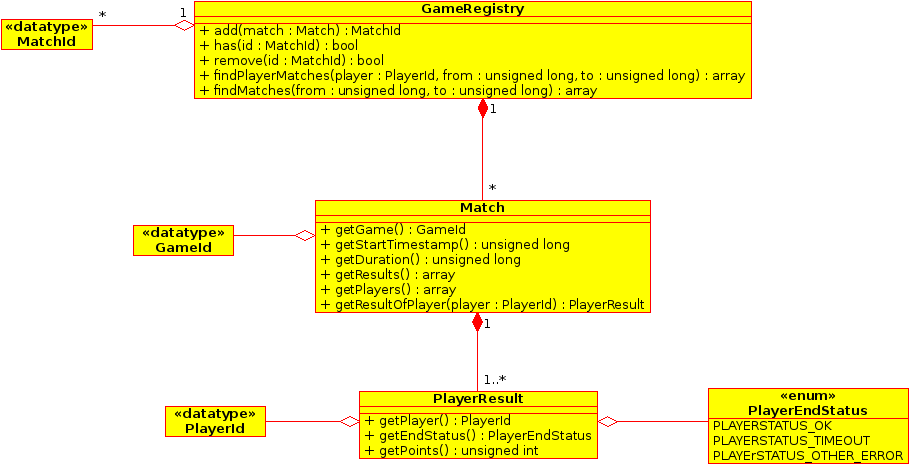
\includegraphics[scale=0.6]{./class_diagram.png}
  % class_diagram.png: 0x0 pixel, 300dpi, 0.00x0.00 cm, bb=
 \end{center}


\section{Arquitectura del sistema}
\begin{figure}[h]
 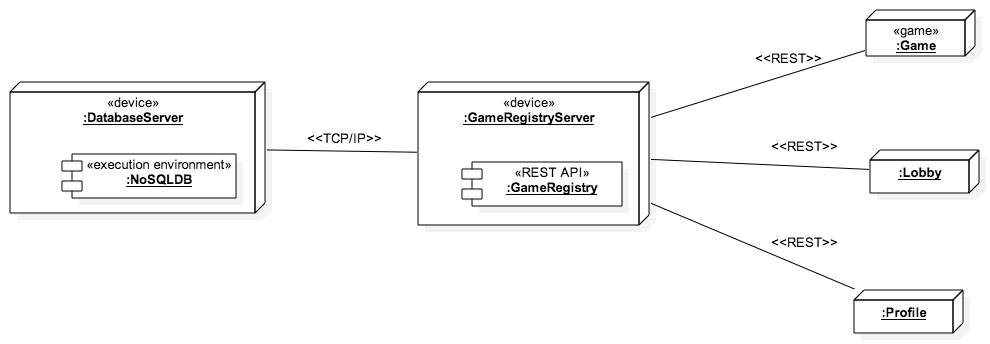
\includegraphics[scale=0.5]{diagrams/deployment_diagram.png}
 \caption{Modelo de despliegue del sistema}
 \label{fig:arquitectura}
\end{figure}


% Tercera iteración (gradle, dockerización)
\chapter{Iteración 3}
\section{Objetivos de iteración}
\begin{itemize}
  \item Integración de Gradle 
  \item Servidor dockerizado
  \item Estructura inicial del Cliente vertx.
\end{itemize}

\section{Gradle}
\emph{Gradle} es un gestor de construcción especialmente indicado para proyectos
Java y con soporte para \emph{Groovy}, \emph{Vertx} y \emph{Maven}.

Ha sido integrado mediante el wrapper \texttt{gradlew} que permite utilizar Gradle sin
instalarlo de forma global en el sistema de desarrollo. La primera vez que se
lanza descargará todas las bibliotecas necesarias.

En el archivo \textbf{Readme.md} hay información básica sobre como construir el
proyecto. Algunos comandos útiles:

\begin{itemize}
 \item Para \textbf{construir} el proyecto: \\
       \texttt{\$ ./gradlew clean modZip}
 \item Para \textbf{lanzar} el servidor en la máquina local: \\
       \texttt{\$ ./gradlew runMod -i}
 \item Para lanzar los \textbf{tests}: \\
       \texttt{\$ ./gradlew clean test}
 \item Para preparar el proyecto para un \textbf{entorno de desarrollo}:
    \begin{itemize}
      \item Eclipse: \texttt{\$ ./gradlew eclipse}
      \item IDEA: \texttt{\$ ./gradlew idea}
    \end{itemize}
\end{itemize}

\section{Dockerización}
\emph{Docker} es una tecnología que permite utilizar contenedores sobre \emph{Linux} para
ejecutar procesos de forma aislada y con un runtime reproducible.

Nuestro proyecto proporciona un archivo \textbf{Dockerfile} con las instrucciones necesarias
para construir el contenedor de la aplicación. Además, el archivo \textbf{Readme.md} contiene
información sobre el procedimiento para lanzar el proyecto en \emph{Docker}. 

El procedimiento para lanzar el servidor con \emph{Docker} ahora mismo es el siguiente:

\begin{itemize}
 \item Limpiar y contruir el proyecto: \\
       \texttt{\$ ./gradlew clean modZip}
 \item Construir el contenedor con el servidor: \\
       \texttt{\$ docker build -t distributedsystems/gameregistry .} \\
       (notar el punto final del comando que indica a \emph{Docker} dónde buscar el archivo
       \emph{Dockerfile} con las instrucciones de construcción). La construcción incluye el 
       resultado de compilación del proyecto por lo que cada vez que este cambie el contenedor
       debe ser reconstruido.
 \item Lanzar el contenedor del servidor: \\
       \texttt{\$ docker run distributedsystems/gameregistry}
\end{itemize}


% Cuarta iteración (mongo, reestructuración de servidor en Servicio / Controlador / Dominio)
%!TEX root =  MemoriaGrupo00.tex
% --------------------------------------------
% Iteraci�n 4
% --------------------------------------------
\chapter{Iteraci�n 4}

\section{Planificaci�n}
\section{Dise�o}
\subsection{Diagrama de clases UML}

\begin{figure}[htbp]
\begin{center}
\missingfigure{Aqu� el modelo de dise�o en formato vectorial preferentemente (pdf)}
% Incluir la figura quitando el comentario a la fila de abajo.
% \includegraphics[width=\textwidth]{myfile.pdf}
\caption{Diagrama UML de dise�o para la iteraci�n 4}
\label{fig:diseno03}
\end{center}
\end{figure}

\subsection{Documentos de asignaci�n de responsabilidades}

\subsection{Memorandos t�cnicos}

\section{Informaci�n adicional}


% Quinta iteración (API inicial, primeros test, despliegue en azure, investigacion integración contínua.
\chapter{Iteración 5}
\section{Objetivos de iteración}
\begin{itemize}
  \item Implementación inicial de API REST
  \item Primeros tests
  \item Despliegue en plataforma Azure
  \item Investigar integración contínua
\end{itemize}


\section{Implementación inicial de API REST}
Hemos definido un primer borrador del API REST a implementar por el servidor. No
es una especificación exhaustiva o completa pero las partes aún no determinadas
de la misma necesitan de información aún no disponible (como por ejemplo las 
necesidades concretas de filtrado de los clientes del servidor).

En siguientes iteraciones queremos integrar la documentación generada por
\emph{Swagger} al final de la memoria. Mientras tanto documento aquí el
borrador actual de la especificación de la API y su implementación actual.

\subsection{API}
El API tiene dos puntos de entrada: \texttt{sessions} y \texttt{session}. 

Todos los recursos responden con contenido \texttt{application/json} con
codificación \texttt{UTF-8}. Los códigos de respuesta HTTP serán siempre
2xx para peticiones correctas, 4xx para errores en la petición y 5xx cuando
hay un error en el servidor.

Toda petición debe incluir dos cabeceras específicas de \emph{GameRegistry}
donde se comunique el identificador de usuario y su token tal y como lo 
validó/generó el \emph{Servidor de Login} del sistema distribuido. Ambos
parámetros serán validados por \emph{GameRegistry} contra el 
\emph{Servidor de Login}.

\subsubsection{/sessions}
Representa una colección de sesiones de juego. Métodos HTTP:

\begin{itemize}
 \item \textbf{GET}: Devuelve una colección de sesiones de juego. Debe aceptar
       parámetros que permitan filtrar la colección. Los parámetros aún no han
       sido definidos (a la espera de conocer las necesidades de los clientes 
       de \emph{GameRegistry}). Devolverá \texttt{200 OK} y una colección de
       sesiones si tiene éxito.
 \item \textbf{POST}: Añade una nueva sesión de juego a la colección. Devolverá
       \texttt{201 Created} si tiene éxito.
 \item \textbf{PUT}: En una especificación REST el comando PUT significa 
       \emph{reemplazar} el recurso con otro. Dicha operación no debe permitirse
       en este contexto por lo que \emph{GameRegistry} devolverá ante peticiones
       como esta el código \texttt{405 Method Not Allowed}.
 \item \textbf{DELETE}: Al igual que PUT, el servidor no debe permitir borrar toda
       la colección de sesiones. Devolverá \texttt{405 Method Not Allowed}.
\end{itemize}

\subsubsection{/sessions/:id}
Representa una única session de juego determinada por su identificador (\texttt{id}). 
Métodos HTTP:

\begin{itemize}
 \item \textbf{GET}: Devuelve la sesión de juego identificada por \texttt{id} con
       código HTTP \texttt{200 OK}. Si no hay sesión con dicho \texttt{id} entonces
       devolverá \texttt{404 Not Found}.
 \item \textbf{POST}: En una especificación REST este comando significa 
       \emph{añadir una nueva entrada a la colección} pero la URL 
       \texttt{/session/:id} no representa una colección sino una única sesión de juego.
       Por tanto este método no tiene sentido y el servidor devolverá 
       \texttt{405 Method Not Allowed}.
 \item \textbf{PUT}: Reemplaza la sesión de juego por la nueva sesión suministrada
       en la petición. Devolverá \texttt{200 OK} o \texttt{404 Not Found} si no hay
       ninguna sesión con ese identificador.
 \item \textbf{DELETE}: Elimina la sesión de juego con el identificador dado. Devolverá
       \texttt{204 No Content} si tiene éxito o \texttt{404 Not Found} si no encuentra
       la sesión de juego.
\end{itemize}

\subsubsection{Otros}
Es muy posible que los requerimientos de los sistemas que dependen de \emph{GameRegistry}
obliguen a implementar nuevos puntos de entrada con comportamientos específicos.


\section{Primeros tests}
Hemos comenzado a escribir una batería de tests automáticos que comprueben el correcto
funcionamiento del servidor.

Los tests incluidos son:

\begin{itemize}
 \item \texttt{testNotFound}: Busca una sesión inexistente, comprueba resultado.
 \item \texttt{testCreate}: Crea una nueva sessión.
 \item \texttt{testUpdate}: Crea una sesión, sube una nueva versión.
 \item \texttt{testDelete}: Crea una sesión, la borra , comprueba que no existe a continuación.
 \item \texttt{testFindSessions}: Crea una sesión y después la busca y comprueba el contador de resultados.
 \item \texttt{testNotAuthenticated}: Intenta una petición sin especificar usuario y token, comprueba error.
\end{itemize}



\section{Despliegue en plataforma Azure}
Tras evaluar las opciones de despliegue de \emph{Docker} en \emph{Azure} hemos
optado por construir una máquina virtual donde administraremos manualmente una
instancia de \emph{Docker} en vez de utilizar la extensión de máquina virtual
que implementa \emph{Azure} para \emph{Docker}. Utilizar esta última habría implicado
una complejidad añadida por la parafernalia necesaria para mantener certificados de
seguridad para poder comunicarnos con la instancia de  \emph{Docker}.

En lugar de la extensión de máquina virtual de \emph{Azure} administraremos la 
máquina virtual manualmente.


\subsection{Test vm}
Para esta iteración hemos creado una máquina virtual cuyo propósito es familiarizarnos
con el entorno \emph{Azure}. Para ello los requisitos de esta máquina serían:

\begin{itemize}
 \item Ser capaz de ejecutar el servidor \emph{GameRegistry} y \emph{MongoDB} como
       contenedores de \emph{Docker}.
 \item Ser capaz de construir el contenedor de \emph{GameRegistry} a partir del 
       repositorio SVN del proyecto.
\end{itemize}

Para ello se ha basado la máquina virtual en una imagen de \emph{Ubuntu 15.04}, que contiene
una versión reciente y razonablemente testada de \emph{Docker}. Además hemos añadido
el cliente de \emph{Subversion} y el \emph{OpenJDK-8}.


\subsection{VM de producción}
Aún no creada. Sus requisitos son similares pero no iguales a la máquina test. El propósito
de esta máquina virtual será el de ejecutar el servidor, evitando la instalación
de cualquier pieza de software no necesaria para esa tarea, lo cual en este caso implica
no instalar ningún \emph{JDK} ni \emph{Subversion}.

Esto requiere algún método para hacer llegar el contenedor con el servidor GameRegistry a
la máquina que no implique a \emph{Subversion} ni el uso de \emph{Java} para compilar
el código fuente. Lo resolveremos en la próxima iteración.

\begin{figure}[h]
 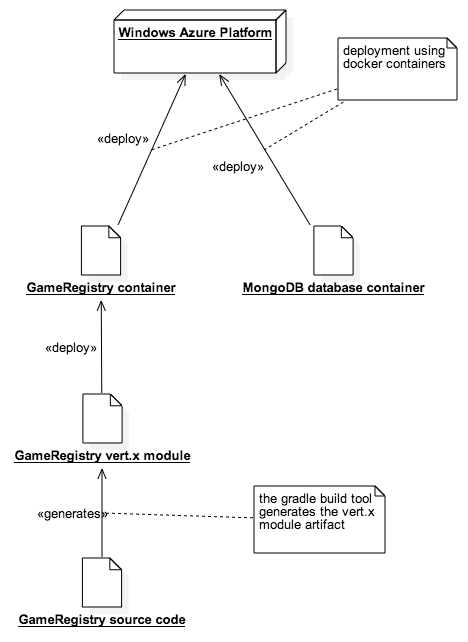
\includegraphics[scale=0.6]{diagrams/docker_deployment_diagram.png}
 \caption{Diagrama de despliegue (iteración 5)}
 \label{fig:despliegue}
\end{figure} 


\section{Investigar integración contínua}
Algún método de integración contínua sería interesante para el proyecto de forma que los tests 
sean ejecutados en cada revisión del proyecto. Hay sitios web que ofrecen una instancia gratuita de
integración contínua que podrían ser utilizados, como por ejemplo:

\begin{itemize}
\item CircleCI (\texttt{https://circleci.com/})
\item CodeShip (\texttt{https://codeship.com/})
\end{itemize}

Estamos aún estudiando la viabilidad y los requisitos impuestos por dichas opciones.
 
\chapter{Iteracion 6}
\section{Objetivos de iteración}
\begin{itemize}
 \item Integración de documentación de Swagger en la memoria y el proyecto.
 \item Testing, integración contínua
\end{itemize} 

\section{Integración de Swagger}
\subsection{Generar la documentación del API REST}
\emph{Swagger} es una especificación que permite documentar servicios REST. Alrededor de
esta especificación existen multitud de herramientas y proyectos que se encargan de
generar dicha documentación a partir de código o de generar otras formas de consumir la
documentación.

Para nuestro caso la generación de la documentación a partir de código, anotaciones, etcétera
no es posible. El tipo de herramientas que genera la documentación se apoyan en \emph{frameworks} 
con estructuras bien definidas para servicios REST, lo que les permite saber cómo extraer esa 
documentación. \emph{Vert.x} es un \emph{framework} de propósito demasiado general como para que 
exista una herramienta capaz de extraer del código de un servidor \emph{Vert.x} dicha información.

Por tanto nos limitaremos a escribir un archivo \emph{Json} con la documentación del servicio
de forma manual.


\subsection{Consumir la documentación}
Hemos desarrollado dos métodos para hacer que la documentación sea accesible para terceros:

\begin{itemize}
 \item Html en el servidor
 \item PDF en la memoria
\end{itemize}


\subsubsection{Html en el servidor}
El proyecto \emph{Swagger-ui} consiste en una serie de archivos \emph{html} y \emph{javascript}
capaces de leer un archivo de documentación \emph{json} de \emph{Swagger} y mostrarla como
\emph{html}, dando incluso la posibilidad de ejecutar peticiones al servicio basándose en
dicha documentación. Para que funcione sólo es necesario suministrarle la URL del archivo
\emph{Json} con la misma.

Para integrarlo en nuestro servicio hemos escrito un pequeño servidor HTTP que se integra con
nuestro servicio a nivel de \emph{RouteMatcher} y sirve el contenido de \emph{Swagger-ui}
bajo un subdirectorio del servidor (\texttt{/doc/}).


\subsubsection{PDF en la memoria}
Utilizando una combinación de los paquetes \emph{npm} y \emph{Bootprint} de \emph{node.js} y
\emph{PhantomJS} somos capaces de generar primero unos archivos HTML describiendo el servicio
REST y después, a partir de estos, un archivo PDF. Todo el proceso esta automatizado a través
de tareas de \emph{Gradle}, siendo necesaria de forma manual unicamente la instalación de 
\emph{PhantomJS} (un motor \emph{Javascript} ``sin navegador'', \emph{headless}).

Dicho archivo PDF es después incluido en la memoria como anexo.


\section{Testing, Integración contínua}
Tras evaluar el servicio \emph{CircleCI} (\texttt{https://circleci.com/}) hemos decidido utilizarlo.

\emph{CircleCI} sólo nos impone tener como VCS \emph{GIT} de forma accesible. Concretamente esta
muy integrado con la plataforma \emph{Git-Hub}, por lo que hemos mudado el desarrollo del proyecto
a dicha plataforma. La url actual del repositorio es: 
\texttt{https://github.com/andihit/dad-gameregistry.git} 

Los datos generales del proyecto han sido actualizados.

Como resultado de la integración, tras el envío de una nueva revisión a \emph{Git-Hub} este
automaticamente (a traves de un \emph{Post-build-hook}) avisa a \emph{CircleCI} de la nueva
revisión y este a su vez descarga el código, lo compila, ejecuta los tests y guarda el informe.


\section{UML actualizado}

El tamaño del diagrama y la lista de argumentos empieza a ser demasiado como para mostrarlo
entero. Obviando los parámetros de las operaciones, sin embargo, la estructura de clases
actual resulta en el siguiente diagrama.

\begin{figure}[h]
 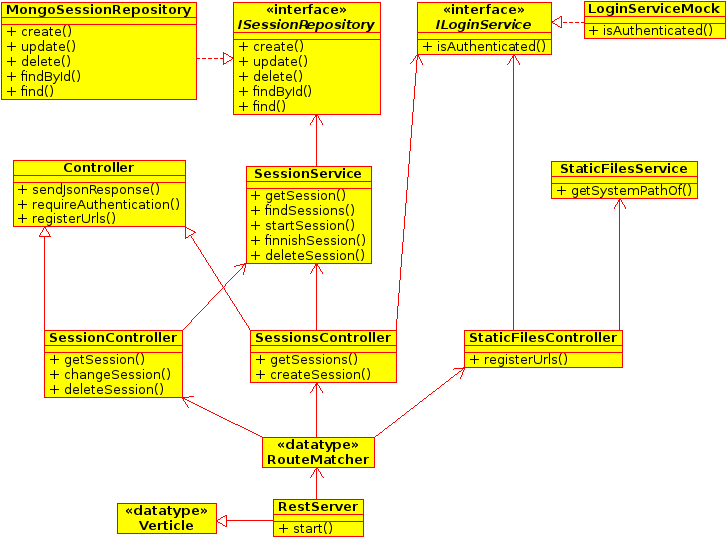
\includegraphics[scale=0.8]{diagrams/class_diagram_iter6.png}
 \caption{Diagrama de clases (iteración 6)}
 \label{fig:clases}
\end{figure} 

\chapter{Iteracion 7}
\section{Objetivos de iteración}
\begin{itemize}
 \item Finalizar cliente de GameRegistry para vertx.
 \item Máquina virtual en producción.
 \item Test sobre \emph{Promises}.
\end{itemize}

 
\section{Finalizar cliente de GameRegistry para vert.x}
El cliente asíncrono para el servidor GameRegistry en Java 
es funcional. En el diseño de la API se ha tenido en
cuenta los siguientes factores:

\begin{itemize}
 \item API con estilo fluído. Debería resultar razonablemente 
       familiar para usuarios de otros objetos Vert.x como 
       \texttt{HttpClient} o \texttt{DnsClient}.
 \item Sin dependencias adicionales. Utilizar el cliente
       no debe obligar al usuario a utilizar más dependencias.
       Esto es lo que ha motivado la elección del lenguaje
       (\emph{Java}) y la ausencia en el diseño de 
       \emph{Lambdas} (obligaría a usar \emph{Java 8})
       o \emph{Promises}.
 \item Simpleza de uso. El cliente siempre devolverá 
       tras una petición y de forma asíncrona un objeto
       \emph{GameRegistryResponse} que contendrá la información
       del resultado, sea un error (con un código de error
       y el \emph{Throwable} causante del error incluído)
       o una colección de sesiones de juego. Sólo requiere,
       por tanto, un manejador (\emph{Handler}) por petición
       y es sencillo detectar el resultado de la petición
       con tan solo comprobar el código de resultado.
 \item Hemos procurado que sea capaz de detectar e informar
       de los errores a través de un código de resultado.
\end{itemize}

Los parámetros de filtrado para peticiones GET a la colección
de sesiones de juego siguen sin especificar y por tanto aún
no están implementados.


\section{Máquina virtual en producción}

El servidor esta funcionando en la plataforma \emph{Azure} sobre
una máquina virtual con el siguiente registro DNS:

\textbf{\texttt{gameregistry.cloudapp.net}}

Nuestro servidor escucha peticiones en el puerto \textbf{8080}.
Para acceder a la documentación de \emph{Swagger} se puede utilizar
la siguiente dirección:

\texttt{http://gameregistry.cloudapp.net:8080/doc/}

La API vive en la siguiente dirección:

\texttt{http://gameregistry.cloudapp.net:8080/api/v1}


\subsection{La máquina virtual}
El sistema de despliegue en estos momentos requiere intervención
manual. Los pasos han sido automatizados en gran medida a través
de \emph{scripts Bash} pero sigue siendo necesario identificarse
en la máquina a través de \emph{ssh} y ejecutar el proceso de
despliegue, dividido en 2 o 3 pasos fundamentales (con sus 
correspondientes \emph{scripts}):

\begin{itemize}
 \item Construcción del contenedor \emph{Docker} del servidor.
 \item Si no esta previamente funcionando, lanzar el contenedor 
       \emph{Docker} de \emph{MongoDB}.
 \item Lanzar el contenedor recién construido del servidor.
\end{itemize}


\section{Test sobre \emph{Promises}}
\subsection{Motivación}
En una sesión de clase el profesor nos indicó que debíamos \emph{demostrar}
que el uso de \emph{Promises} en nuestro servidor no bloqueaba el hilo principal
de \emph{Vert.x}. Dado que es una tarea encargada a nuestro
grupo de forma particular vamos a entrar en más detalle del normal en 
la cuestión.

En nuestro servidor utilizamos \emph{Promises} para hacer más legible y sencilla
la programación asíncrona de algunos de los servicios internos (como el servicio
de autenticación que debe validar con el \emph{LoginServer} los pares 
usuario-token de las peticiones realizadas a nuestro servidor). En concreto utilizamos
una implementación para \emph{Groovy}:

\texttt{com.darylteo.vertx:vertx-promises-groovy:1.2.1}

Dicha biblioteca establece en su \texttt{Readme} la siguiente información:

\say{Esta biblioteca implementa la mayor parte de la especificación 
\emph{Promises/A+}. Esta basado en \emph{Q} para \emph{Node.js}, que añade
facilidades adicionales como \texttt{reject} y \texttt{finally}. Finalmente,
esta construida utilizando la biblioteca \emph{RxJava}.}

También menciona la siguiente información:

\say{Esta biblioteca no se parece a otras implementaciones similares basadas
en lenguaje (como \emph{Futures} o \emph{GroovyPromise} en tanto a que
esta completamente libre de bloqueos. Esta diseñada para trabajar con
plataformas que hacen uso intensivo de \emph{callbacks} asíncronos. Es más,
tiene varias clases adicionales que intentan mejorar la seguridad de tipos
del uso basado en \emph{Java} a la vez que minimiza el exceso de \emph{verbosidad}
a través de la inferencia de \emph{generics}.

Por tanto es de esperar que seamos capaces de demostrarlo con un test razonablemente
simple.}

\subsection{El test}
La secuencia del test es la siguiente:

\begin{itemize}
 \item Lanzar desde el test una petición con un \emph{path} específico al servidor.
 \item El servidor, en respuesta a esta petición al \emph{path} específico,
       debe utilizar un \emph{Timer} de \emph{Vert.x} para retrasar su respuesta
       artificialmente un cierto tiempo (20 segundos). Para que el test
       demuestre que \emph{Promises no bloquea} el \emph{Timer} debe iniciarse
       desde dentro de un método que devuelve una \emph{promesa} que sólo será
       cumplida desde el código invocado por el \emph{Timer} al terminar la
       espera.
 \item Un cierto tiempo después de la primera petición el test debe lanzar una
       segunda petición a un \emph{path} del servidor con comportamiento normal
       de forma que este responda antes de que el tiempo de espera artificial
       de la primera petición se cumpla.
 \item Finalmente, el test debe recibir la respuesta a la segunda petición y
       al cabo de 20 segundos de lanzar la primera petición debe recibir la respuesta
       a esta.
\end{itemize}

\subsubsection{Implementación}

En el lado del servidor el código de inicialización del \emph{RouteMatcher} añade
de forma opcional (según el contenido de \emph{conf.json}) una ruta adicional 
con un manejador simple que llama a un nuevo servicio interno llamado
\emph{DebugPromiseService}, que a través de una \emph{promesa} devuelve una
cadena de texto que se utilizará en la respuesta. Más adelante en esta iteración
hay un diagrama de clases actualizado que muestra la estructura general del mismo.

A continuación se muestra el código pertinente del servicio (\emph{Groovy}):

\begin{verbatim}
 Promise<String> doSomething(HttpServerRequest request) {
   final Promise<HttpServerResponse> p = new Promise()

   vertx.setTimer(wait_time * 1000, { time ->
     p.fulfill("<html><body>Waited " 
               + wait_time 
               + " seconds to give this answer.</body></html>")
   })

   return p;
 }
\end{verbatim}

El test tiene la siguiente implementación:

\begin{verbatim}
 def testDebugPromiseIsNotBlocking() {
   HttpClient client = vertx.createHttpClient().setPort(8080)
   HttpClient client2 = vertx.createHttpClient().setPort(8080)
   String path = "/debug_promise"
   List<Integer> order = []

   // This gets the first request going
   container.logger.info("#1: Launching first request!")
   order.add(1)

   client.getNow(path, { response ->
     // This code will execute around 20 secs after the 
     // getNow call was performed
     container.logger.info("#4: First request answered.")
     order.add(4)

     assertEquals([1,2,3,4], order)
     testComplete()
   })

   // Wait for 2 seconds
   vertx.setTimer(2 * 1000, {long time ->
     // And then do another request that should end 
     // before the first one.
     container.logger.info("#2: Launching second request!")
     order.add(2)

     client2.getNow("/doc", { response ->
       container.logger.info("#3: Second request answered.")
       order.add(3)
     })
   })
  }
\end{verbatim}

Cabe destacar que la implementación de \texttt{HttpClient} no es capaz de realizar
dos peticiones simultaneas al mismo host en el mismo \emph{verticle}. Resultaba confuso 
porque los resultados del test parecían sugerir que efectivamente el servidor estaba 
bloqueando tras la primera petición pero realmente era el cliente Http el problema. 
Con dos instancias del cliente Http el test pasa sin problemas.


\section{Diagrama UML actualizado}

Se incluyen diagramas UML tanto del servidor como del cliente en su estado actual.

\begin{figure}[h]
 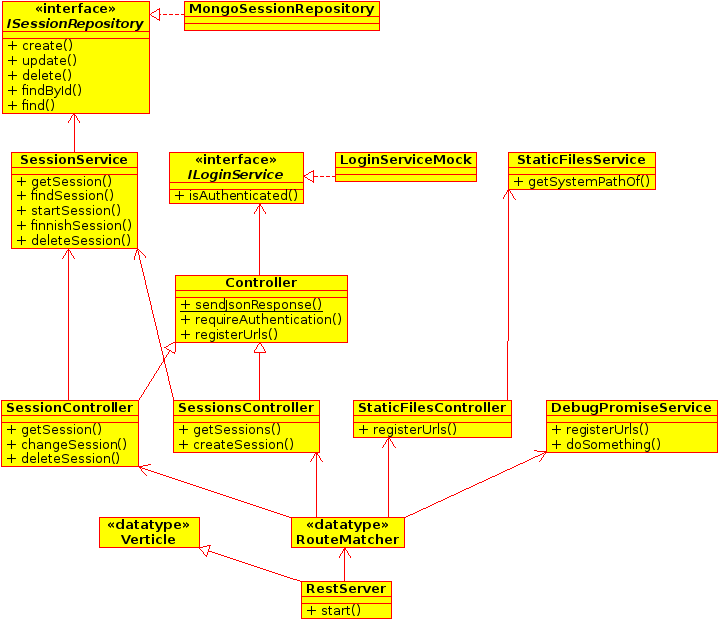
\includegraphics[scale=0.8]{diagrams/class_diagram_iter7.png}
 \caption{Diagrama de clases (iteración 7)}
 \label{fig:clases}
\end{figure} 

\begin{figure}[h]
 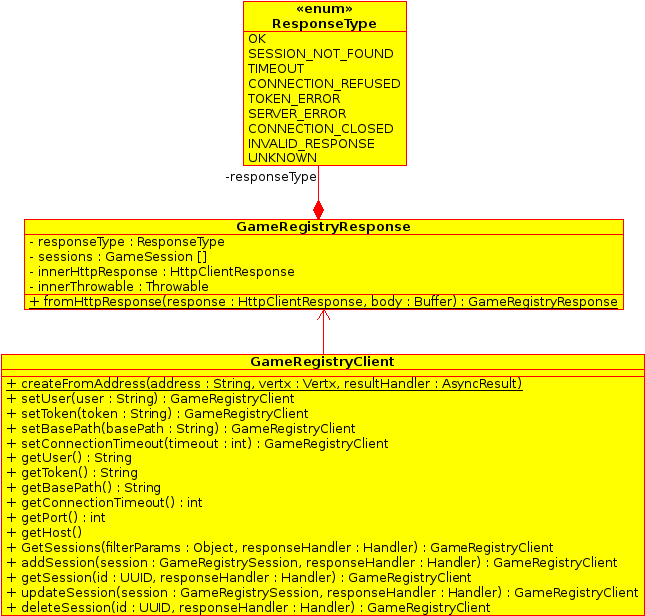
\includegraphics[scale=0.8]{diagrams/class_diagram_client_iter7.png}
 \caption{Diagrama de clases del cliente (iteración 7)}
 \label{fig:clases}
\end{figure} 



\chapter{Documentación de API GameRegister}
\includepdf[pages={-}]{../gameregistry/build/docs/apidoc/pdf/apidoc.pdf}

\end{document}
